\documentclass[a4paper,12pt]{article}

% Основные пакеты
\usepackage[utf8]{inputenc}             % Поддержка кодировки UTF-8
\usepackage[T1, T2A]{fontenc}           % Поддержка кириллицы
\usepackage[english, russian]{babel}    % Поддержка русского и английского языков
\usepackage{graphicx}                   % Для вставки изображений
\usepackage{import}                     % Для продвинутого импорта (например, из Inkscape)
\usepackage{subcaption}                 % Для создания подписей к изображениям в сетке
\usepackage{float}                      % Для улучшенного размещения изображений
\usepackage{geometry}                   % Для управления отступами на странице
\usepackage{amsmath, amssymb, amsfonts} % Для математических формул и символов
\usepackage{booktabs}                   % Для красивых таблиц
\usepackage[dvipsnames]{xcolor}         % Для расширенной поддержки цветов
\usepackage[colorlinks]{hyperref}       % Для создания гиперссылок
\usepackage{indentfirst}                % Для красной строки в первом абзаце
\usepackage{listings}                   % Для оформления листингов кода
\usepackage{longtable}                  % Для длинных таблиц
\usepackage{makecell}                   % Для улучшенного форматирования ячеек таблиц
\usepackage{multirow}                   % Для объединения строк в таблицах
\usepackage{tabularray}                 % Для продвинутых таблиц
\usepackage{varwidth}                   % Для переменной ширины блоков
\usepackage{bm}                         % Для жирных математических символов
\usepackage{pifont}                     % Для специальных символов (например, галочек)
\usepackage{fontawesome}                % Для иконок
\usepackage{tcolorbox}
% Настройка отступов на странице
\geometry{left=2cm, right=2cm, bottom=2cm, top=2cm}

% Настройка гиперссылок
\hypersetup{
	linkcolor=blue,
	filecolor=magenta,
	urlcolor=cyan
}

% Настройка листингов
\definecolor{codegreen}{rgb}{0,0.6,0}
\definecolor{codegray}{rgb}{0.5,0.5,0.5}
\definecolor{codepurple}{rgb}{0.58,0,0.82}
\definecolor{backcolour}{rgb}{0.95,0.95,0.92}

% Определим стиль для выделения переменных
\lstdefinestyle{codestyle}{
	backgroundcolor=\color{backcolour},  % Цвет фона
	commentstyle=\color{codegreen}\itshape,  % Стиль для комментариев
	keywordstyle=\color{magenta}\bfseries,  % Стиль для ключевых слов
	numberstyle=\tiny\color{codegray},  % Стиль для номеров строк
	stringstyle=\color{codepurple},  % Стиль для строк
	identifierstyle=\color{black},  % Стиль для переменных (выделим их синим)
	basicstyle=\ttfamily\footnotesize,  % Размер шрифта для кода
	breakatwhitespace=false,  % Не разрывать строки в пробелах
	breaklines=true,  % Разбивать длинные строки
	captionpos=b,  % Позиция заголовка (внизу)
	keepspaces=true,  % Сохранять пробелы
	numbers=left,  % Позиция номеров строк
	numbersep=10pt,  % Расстояние между кодом и номерами строк
	showspaces=false,  % Не показывать пробелы
	showstringspaces=false,  % Не показывать пробелы в строках
	showtabs=false,  % Не показывать табуляции
	tabsize=4,  % Размер табуляции
	frame=single,  % Добавить рамку вокруг кода
	rulecolor=\color{black},  % Цвет рамки
	backgroundcolor=\color{backcolour},  % Цвет фона рамки
	xleftmargin=15pt,  % Отступ слева
	xrightmargin=15pt,  % Отступ справа
}

\lstset{style=codestyle, extendedchars=\true}


\begin{document}
	\begin{titlepage}
		\centering
		\vspace*{1cm}
		
		{\large Министерство науки и высшего образования Российской Федерации}\\
		{\large ФЕДЕРАЛЬНОЕ ГОСУДАРСТВЕННОЕ АВТОНОМНОЕ ОБРАЗОВАТЕЛЬНОЕ УЧРЕЖДЕНИЕ ВЫСШЕГО ОБРАЗОВАНИЯ «НАЦИОНАЛЬНЫЙ ИССЛЕДОВАТЕЛЬСКИЙ УНИВЕРСИТЕТ ИТМО»}\\
		{\large (УНИВЕРСИТЕТ ИТМО)}\\
		
		\vspace{2cm}
		
		{\large Факультет «Систем управления и робототехники»}\\
		
		\vspace{3cm}
		
		\textbf{{\Huge ОТЧЕТ}\\
			{\Huge О ЛАБОРАТОРНОЙ РАБОТЕ №4}}\\
		
		\vspace{1cm}
		
		{\LARGE По дисциплине «Техническое зрение»}\\
		{\LARGE на тему: «Сегментация изображений»}\\
		
		\vspace{2cm}
		
		{\Large Студент:}\\
		Охрименко Ева ИСУ 409290\\
		
		\vspace{2cm}
		
		{\Large Преподаватель:}\\
		Шаветов Сергей Васильевич\\
		
		\vspace{5cm}
		
		{\large г. Санкт-Петербург}\\
		{\large 2025}
		
	\end{titlepage}
	
	\tableofcontents  % Оглавление
	\newpage
	
	\section*{Цель работы}
	\addcontentsline{toc}{section}{Цель работы} 
	
Освоение основных способов фильтрации изображений от шумов и выделения контуров.

	\section{Task. Типы шумов}
	В этом задании мне нужно обработать мое изображение различными шумами.
	
	\begin{figure}[H]
		\centering
		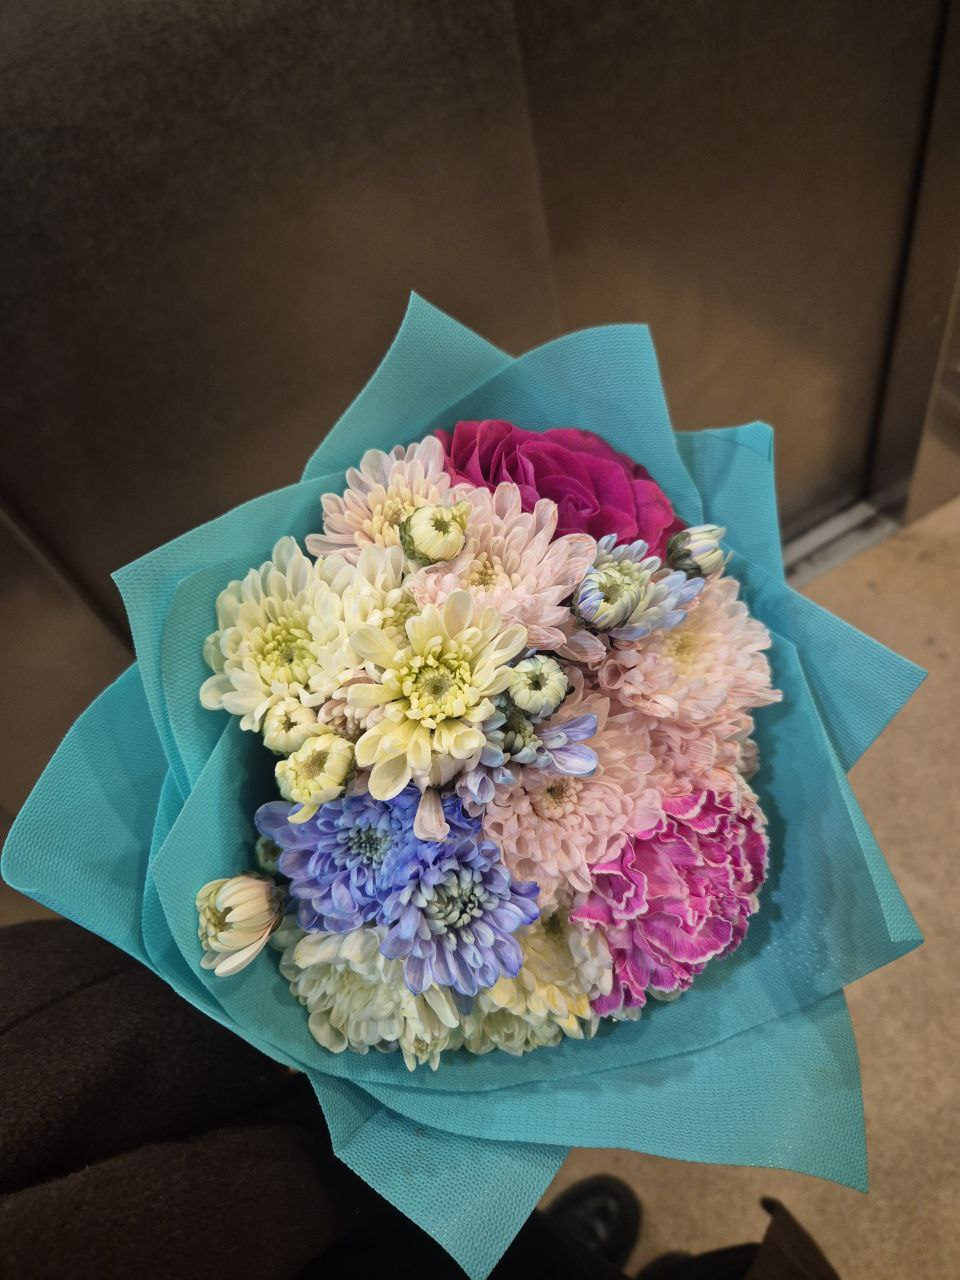
\includegraphics[width=0.5\linewidth]{../images/flowers.jpg}
		\caption{Исходное изображение} 
	\end{figure}
	
	
	
	\subsection{Импульсный шум}
	
	Способ накладывания шума: берем пиксель и меняем его интенсивность на значение $d \in [0,255]$ с вероятностью \texttt{P} - передаваемый параметр в функцию.
	\[
	I(x,y) = 
	\begin{cases} 
		d, & \text{c вероятностью } p, \\ 
		s_{x,y}, & \text{c вероятностью } (1-p), 
	\end{cases}
	\]
	
	\begin{lstlisting}[language=python, caption={Функция накладывания импульсного шума}]
def imNoise(image, amount=0.5):
	noisy_image = random_noise(image, mode="s&p", amount=amount)
	noisy_image = (noisy_image * 255).astype(np.uint8)
	return noisy_image
\end{lstlisting}

	Полученное изображение:
	
		\begin{figure}[H]
		\centering
		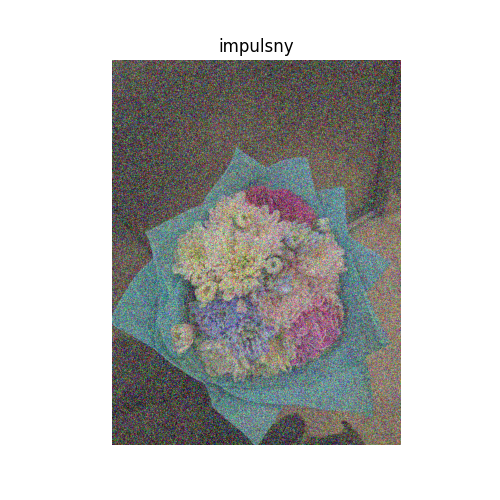
\includegraphics[width=0.5\linewidth]{../noise/impuls.png}
		\caption{Изображение с импульсным шумом} 
	\end{figure}

	
	
	\subsection{Аддитивный шум}
	
Аддитивный шум описывается следующим выражением:

\[
I_{\text{new}}(x,y) = I(x,y) + \eta(x,y)
\]

где $I_{\text{new}}$ — зашумленное изображение, $I$ — исходное изображение,  
$\eta$ — не зависящий от сигнала аддитивный шум с гауссовым или любым другим распределением функции плотности вероятности.

	\begin{lstlisting}[language=python, caption={Функция накладывания аддитивного шума}]
def addNoise(image, noise):
	noisyImage = image + noise
	return np.clip(noisyImage, 0, 255).astype(np.uint8)
\end{lstlisting}

	Полученное изображение. Параметр \texttt{noise = 100}:

\begin{figure}[H]
	\centering
	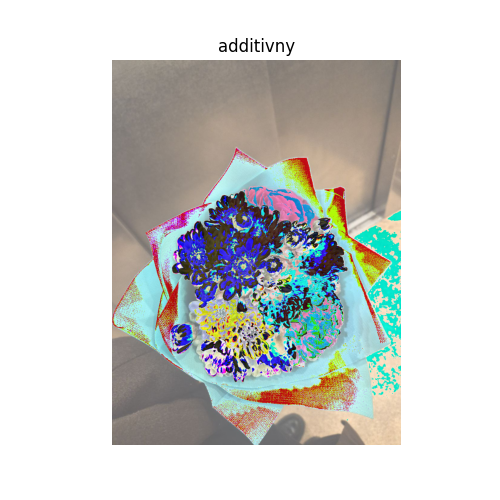
\includegraphics[width=0.44\linewidth]{../noise/additive.png}
	\caption{Изображение с аддитивным шумом} 
\end{figure}

\subsection{Мультипликативный шум}

Мультипликативный шум описывается следующим выражением:

\[
I_{\text{new}}(x,y) = I(x,y) \cdot \eta(x,y)
\]

где $I_{\text{new}}$ — зашумленное изображение, $I$ — исходное изображение,  
$\eta$ — не зависящий от сигнала мультипликативный шум, умножающий зарегестрированный сигнал.

\begin{lstlisting}[language=python, caption={Функция накладывания мультипликативного шума}]
def mulNoise(image, noise):
	noisyImage = image * noise
	return np.clip(noisyImage, 0, 255).astype(np.uint8)
\end{lstlisting}

Полученное изображение. Параметр \texttt{noise = 5}:

\begin{figure}[H]
	\centering
	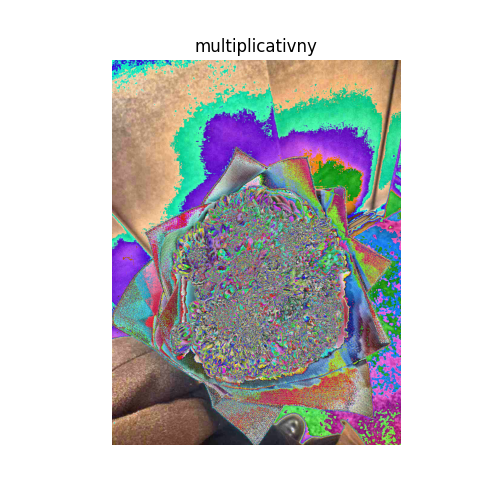
\includegraphics[width=0.5\linewidth]{../noise/multiplicativny.png}
	\caption{Изображение с аддитивным шумом} 
\end{figure}

\subsection{Гауссов (нормальный) шум}



Гауссов шум на изображении может возникать вследствие недостатка освещенности сцены, высокой температуры и т.д. Модель шума широко распространена в задачах низкочастотной фильтрации изображений. Функция распределения плотности вероятности $p(z)$ случайной величины $z$ описывается выражением:

\begin{equation}
	p(z) = \frac{1}{\sigma\sqrt{2\pi}} e^{-\frac{(z-\mu)^2}{2\sigma^2}},
	\label{eq:gauss_noise}
\end{equation}

где $z$ — интенсивность изображения ($z \in [0,255]$), $\mu$ — среднее, $\sigma$ — СКО. 


\begin{lstlisting}[language=python, caption={Функция накладывания гауссова шума}]
def gayNoise(img, mean, var):
	noise = np.random.normal(mean, var**0.5, img.shape)
	return np.clip(img + noise * (255 if img.dtype == np.uint8 else 1), 0, 255).astype(img.dtype)
\end{lstlisting}

Полученное изображение. Параметры \texttt{mean = 1, var = 12}:

\begin{figure}[H]
	\centering
	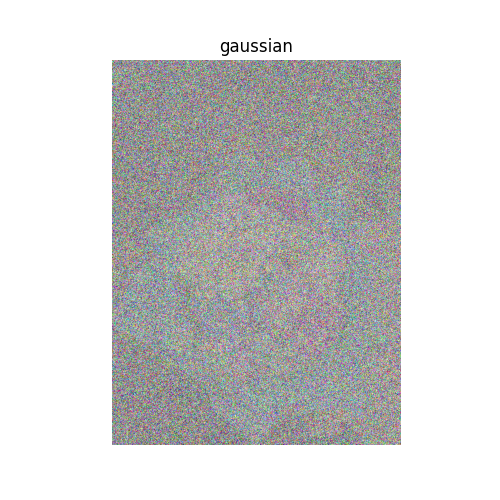
\includegraphics[width=0.5\linewidth]{../noise/gaussian.png}
	\caption{Изображение с нормальным шумом} 
\end{figure}

\subsection{Шум квантования}

Зависит от выбранного шага квантования и самого сигнала. Шум квантования может приводить, например, к появлению ложных контуров вокруг объектов или убирать слабоконтрастные детали на изображении. Такой шум не устраняется.


\begin{lstlisting}[language=python, caption={Функция накладывания шума} квантования]
def kvantNoise(img):
	rng = np.random.default_rng()
	if img.dtype == np.uint8:
		img = img.astype(float) / 255
		noisy = rng.poisson(img * 2) / 2
		noisy = (255 * noisy.clip(0, 1)).astype(np.uint8)
	else:
		noisy = rng.poisson(img * 2) / 2
	
	return noisy
\end{lstlisting}

Полученное изображение.

\begin{figure}[H]
	\centering
	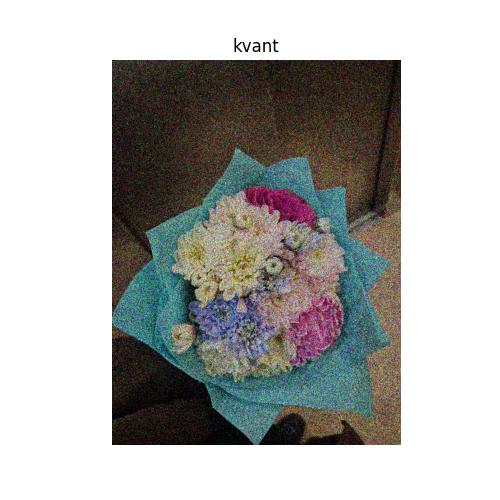
\includegraphics[width=0.5\linewidth]{../noise/kvant.png}
	\caption{Изображение с квантовым шумом} 
\end{figure}

	\section{Task. Низкочастотная фильтрация}
	
	В этом задании мне нужно обработать полученные в предыдущем пункте искаженные изображения фильтром Гаусса и контргармоническим усредняющим фильтром с различными значениями параметра $Q$.
	
	\subsection{Гауссов фильтр}
	Фильтр Гаусса применяет весовую функцию к пикселям в окрестности:
	\[ G_{\sigma}(x,y) = \frac{1}{2\pi\sigma^2} e^{-\frac{x^2 + y^2}{2\sigma^2}} \]
	где \(\sigma\) — параметр размытия. Чем больше \(\sigma\), тем сильнее сглаживание.
	
	\begin{lstlisting}[language=python, caption={Фильтр Гаусса}]
def gaus(image, q):
	filtered = gaussian(image, sigma=abs(q), preserve_range=True)
	filtered = np.clip(filtered, 0, 255).astype(np.uint8)
	return filtered
\end{lstlisting}

Применю фильтр к своим зашумленным изображениям. Возьму \( Q \in \{-1, 0, 1\} \).

\begin{itemize}
	\item Импульсный шум
		\begin{figure}[H]
			\centering
			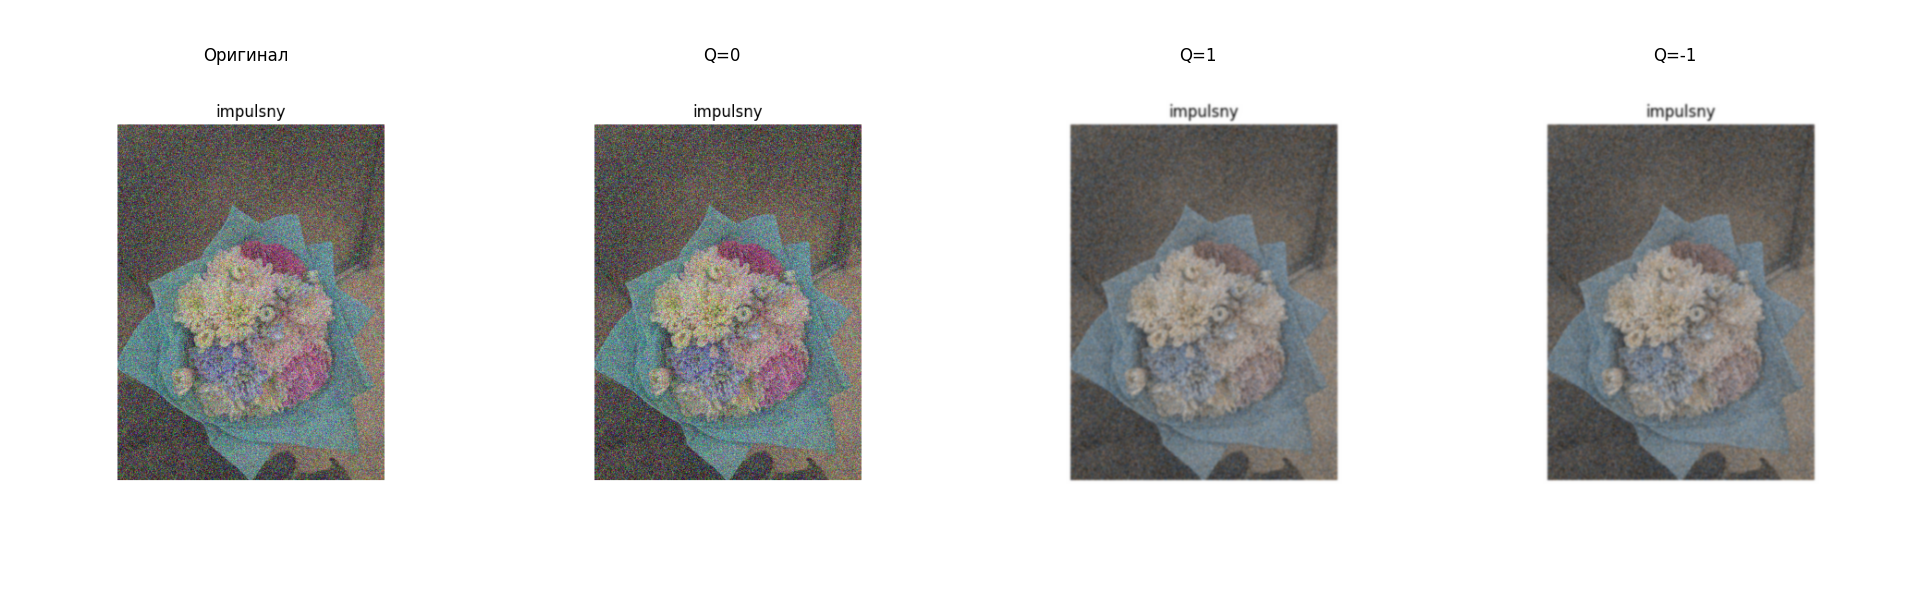
\includegraphics[width=1\linewidth]{../filtreted/fImp.png}
		\end{figure}
		
	\item Аддитивный шум
	\begin{figure}[H]
		\centering
		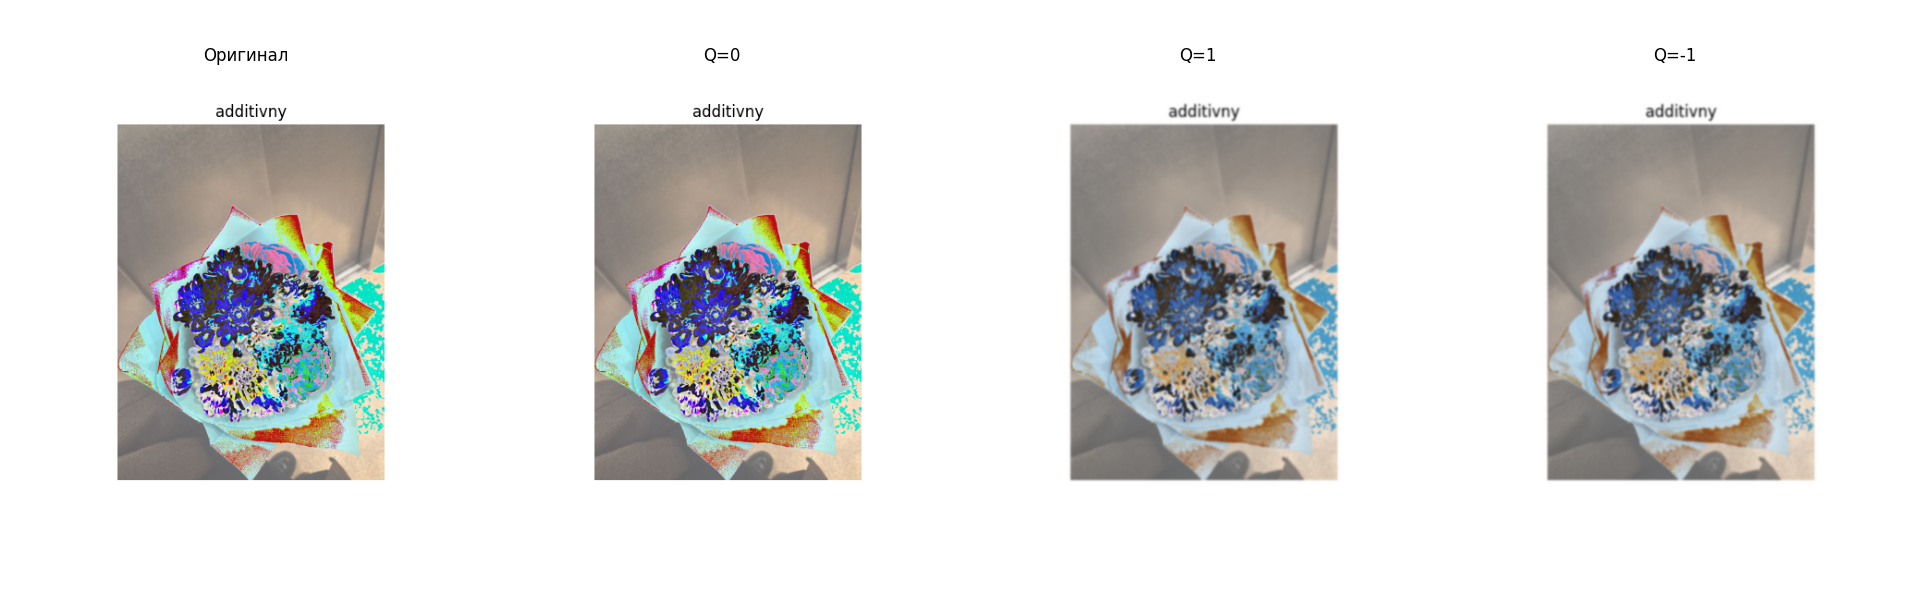
\includegraphics[width=1\linewidth]{../filtreted/fAdd.png}
	\end{figure}
	
	\item Мультипликативный шум
	\begin{figure}[H]
		\centering
		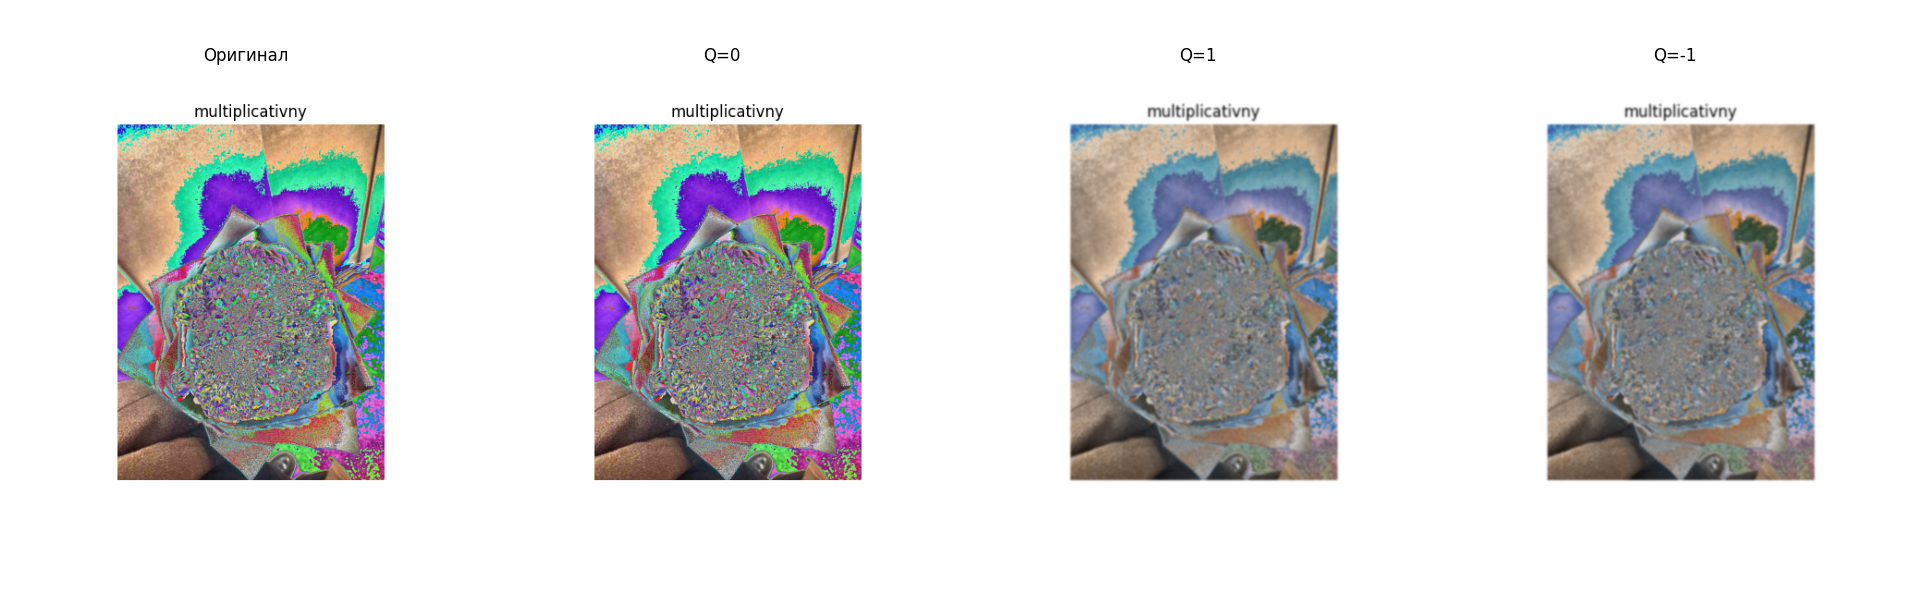
\includegraphics[width=1\linewidth]{../filtreted/fMul.png}
	\end{figure}
	
	\item Шум квантования
	\begin{figure}[H]
		\centering
		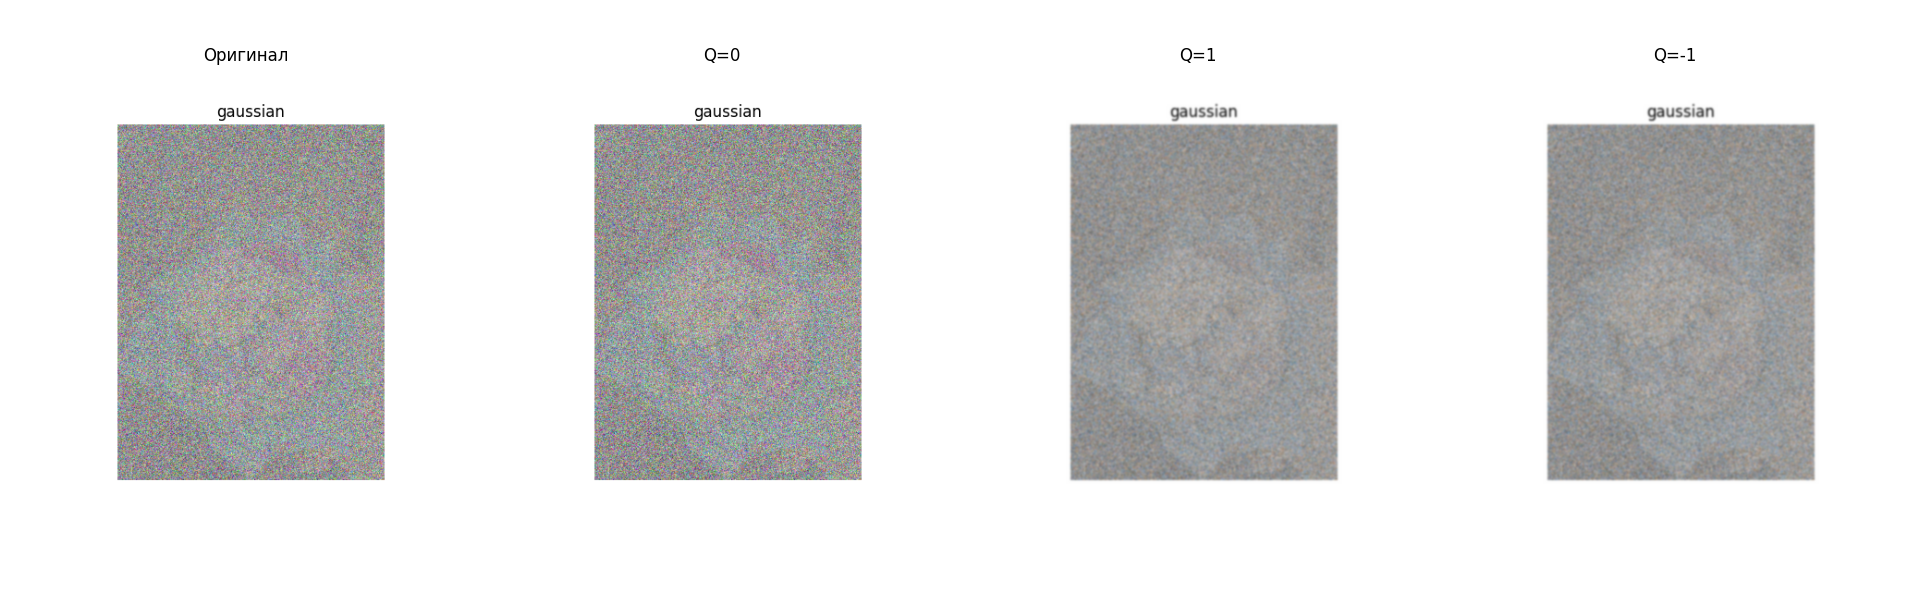
\includegraphics[width=1\linewidth]{../filtreted/fGay.png}
	\end{figure}
	
	\item Импульсный шум
	\begin{figure}[H]
		\centering
		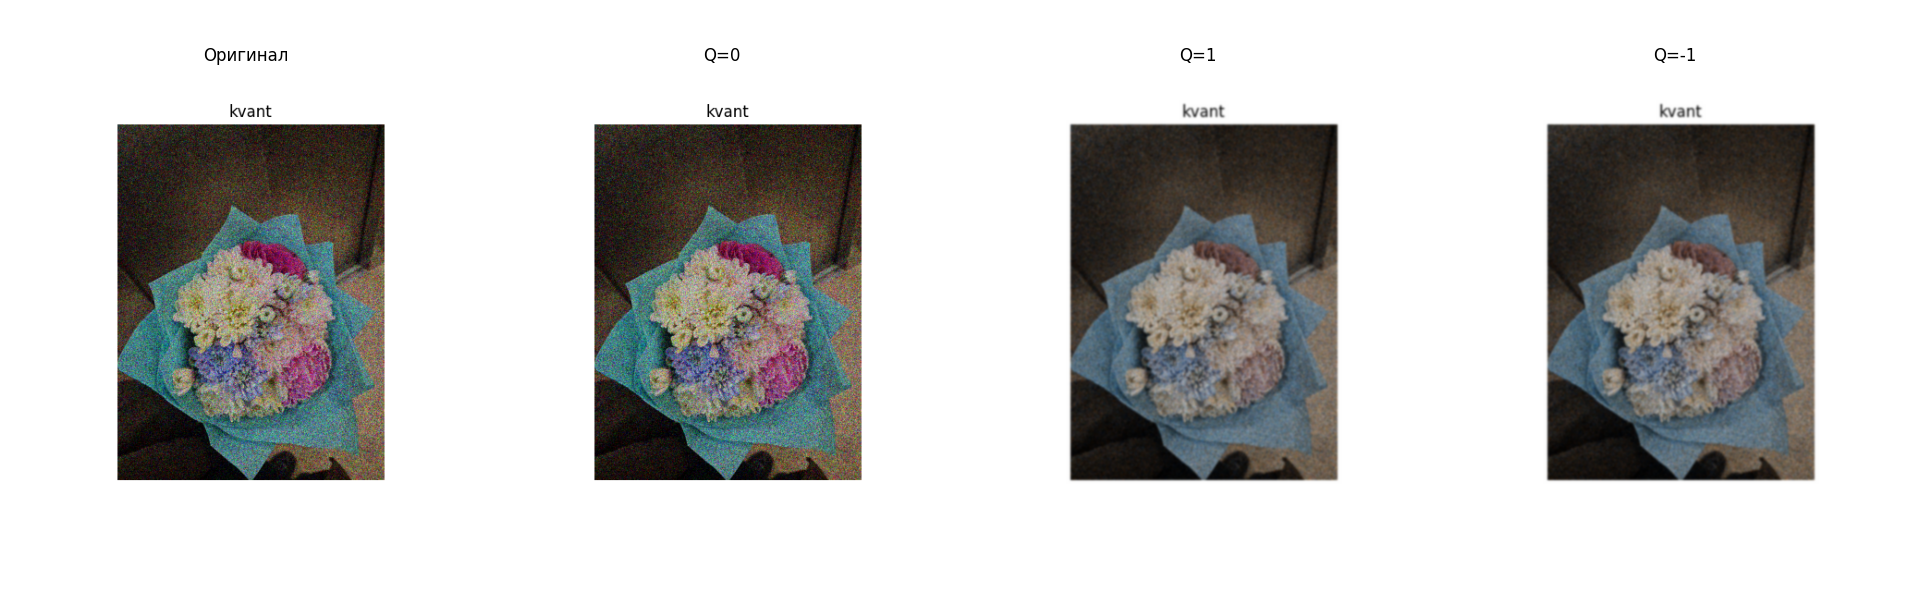
\includegraphics[width=1\linewidth]{../filtreted/fKva.png}
	\end{figure}
\end{itemize}
Можно заметить, что изображения размываются.
	
	\subsection{Контргармонический усредняющий фильтр}
	
Контргармонический фильтр определяется как:

\[
I_{\text{new}}(x,y) = \frac{\sum\limits_{i,j} I(i,j)^{Q+1}}{\sum\limits_{i,j} I(i,j)^Q}
\]

где:
\begin{itemize}
	\item $Q > 0$ подавляет шум типа <<перец>>
	\item $Q < 0$ подавляет шум типа <<соль>>
	\item $Q = 0$ даёт арифметическое среднее
	\item $Q = -1$ даёт гармоническое среднее
\end{itemize}

\begin{lstlisting}[language=python, caption={Контргармонический усредняющий фильтр}]
def contraharmonicMean(img, q=0, kernel_size=3):
	img_float = img.astype(np.float32) + 1e-10
	if q == 0:
		return img
	
	kernel = np.ones((kernel_size, kernel_size), np.float32)
	numerator = cv2.filter2D(np.power(img_float, q + 1), -1, kernel)
	denominator = cv2.filter2D(np.power(img_float, q), -1, kernel)
	filtered = np.zeros_like(img_float)
	np.divide(numerator, denominator, out=filtered, where=denominator!=0)
	return np.clip(filtered, 0, 255).astype(np.uint8)
\end{lstlisting}
	

Применю фильтр к своим зашумленным изображениям. Возьму \( Q \in \{-1, 0, 1\} \).

\begin{itemize}
	\item Импульсный шум
	\begin{figure}[H]
		\centering
		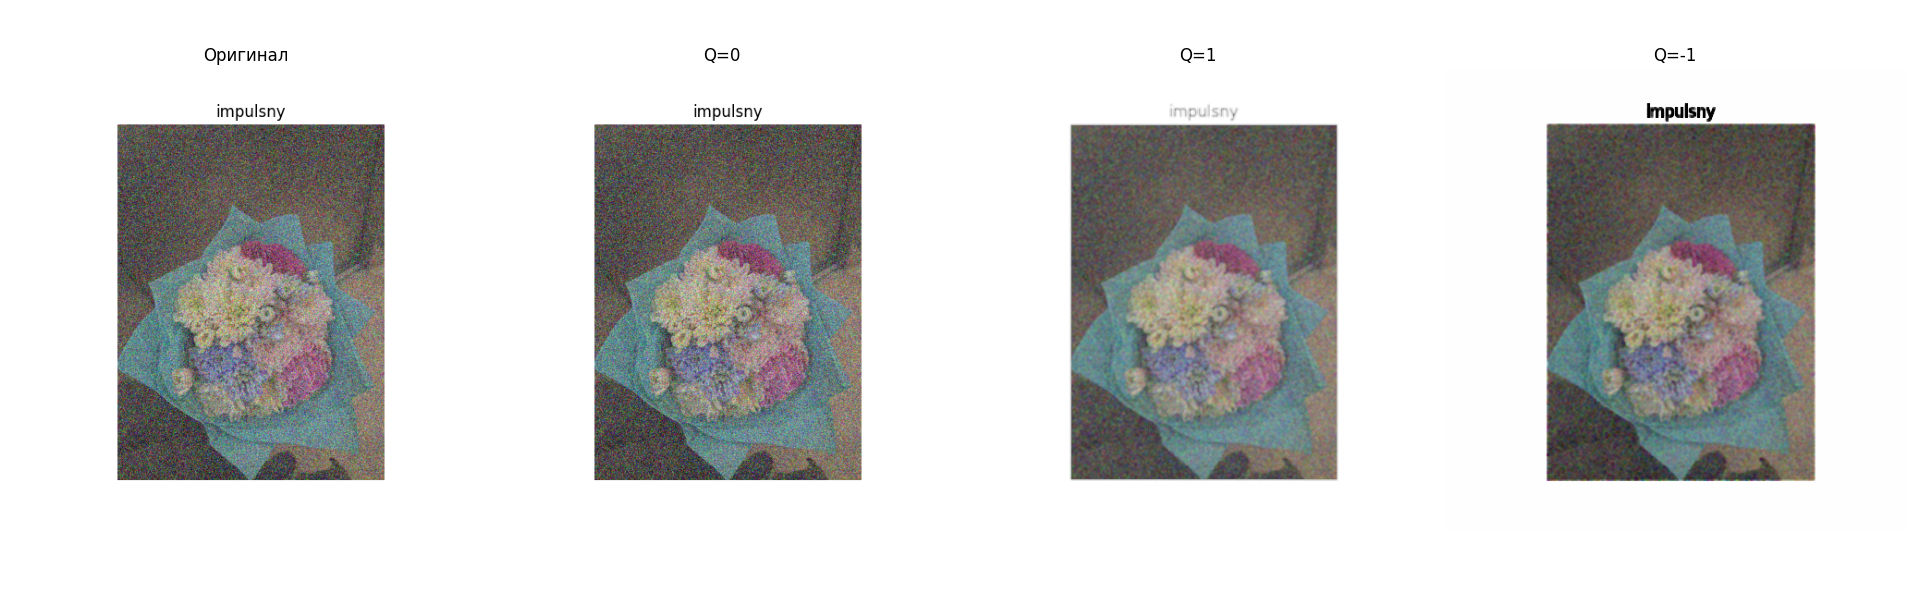
\includegraphics[width=1\linewidth]{../filtreted/kfImp.png}
	\end{figure}
	
	\item Аддитивный шум
	\begin{figure}[H]
		\centering
		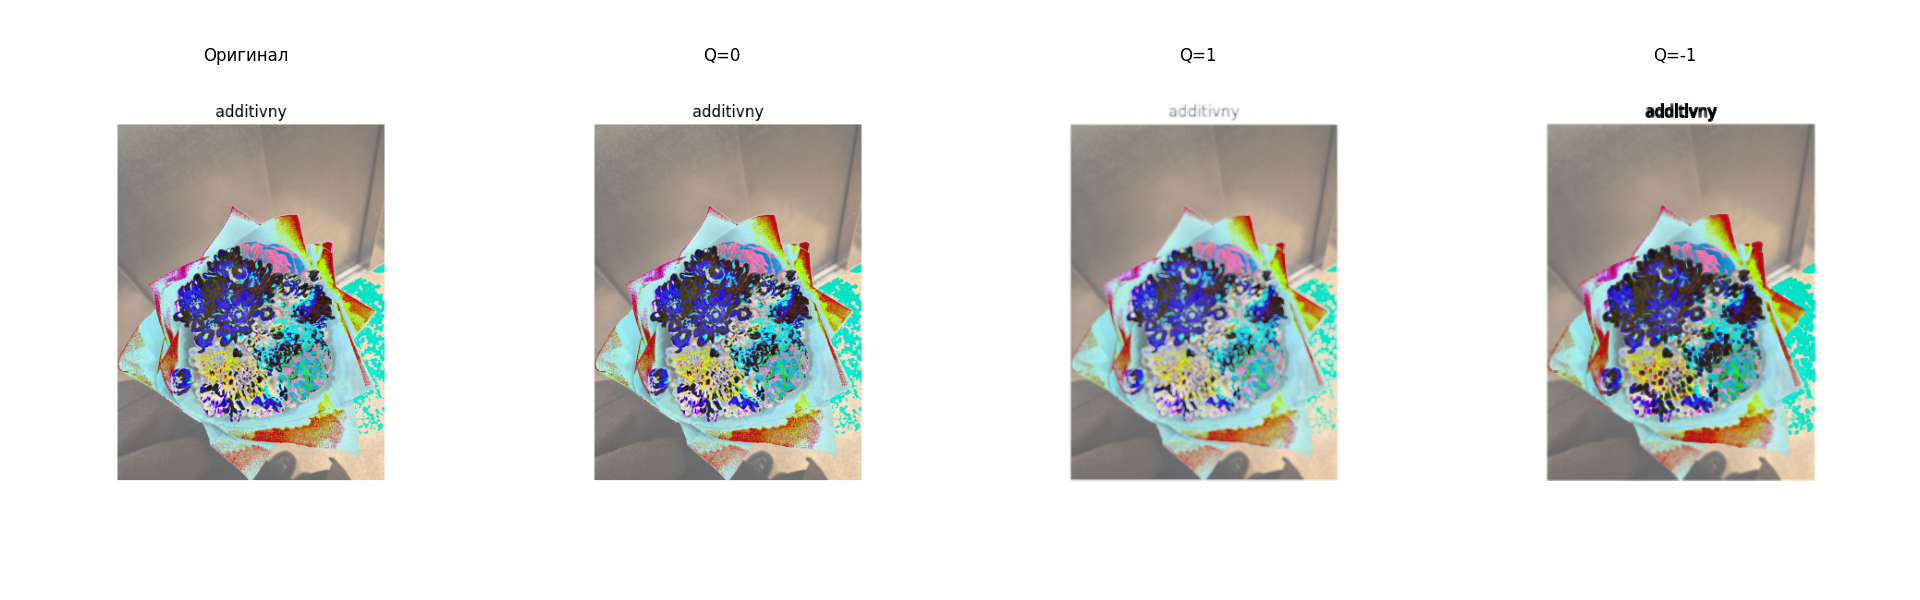
\includegraphics[width=1\linewidth]{../filtreted/kfAdd.png} 
	\end{figure}
	
	\item Мультипликативный шум
	\begin{figure}[H]
		\centering
		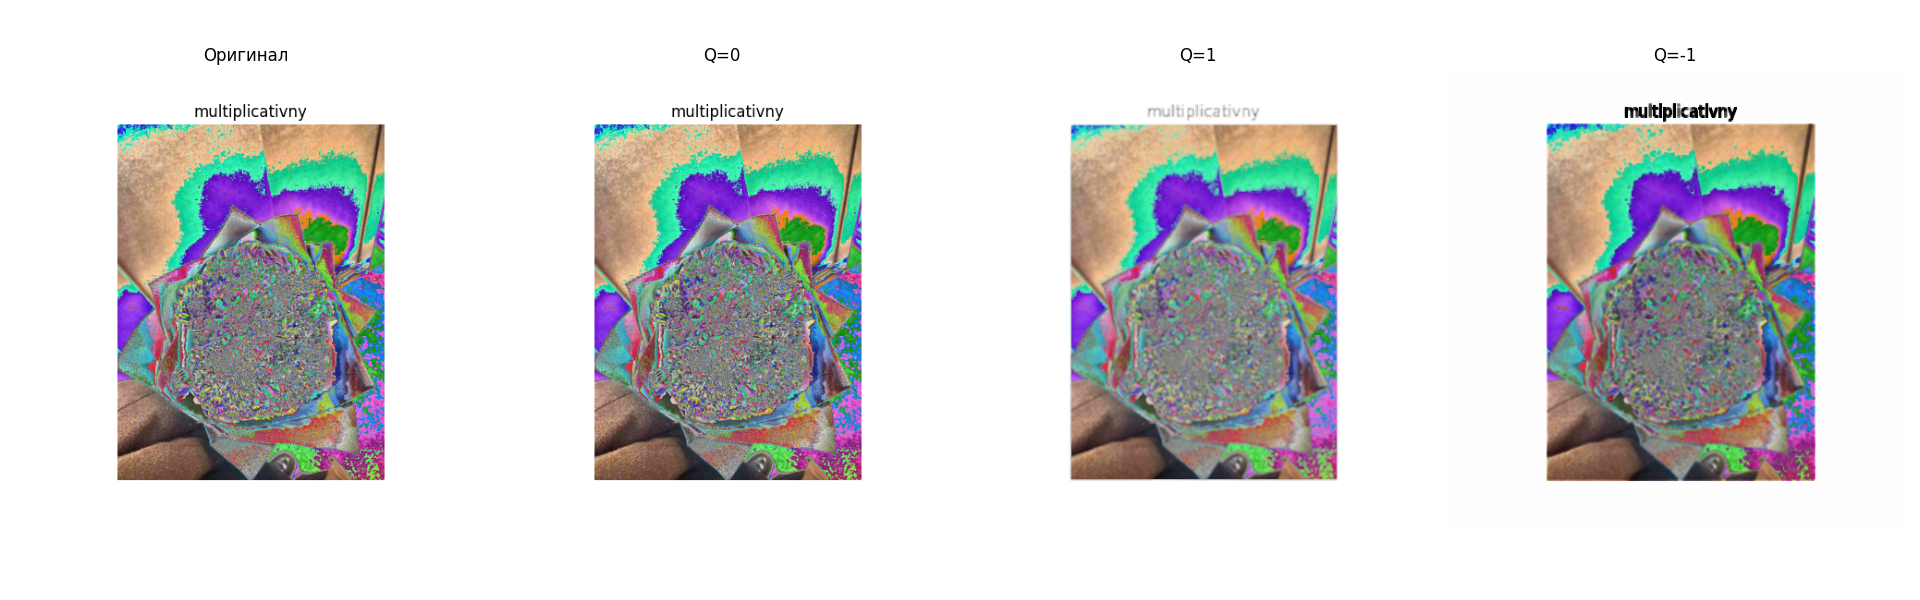
\includegraphics[width=1\linewidth]{../filtreted/kfMul.png}
	\end{figure}
	
	\item Шум гаусса
	\begin{figure}[H]
		\centering
		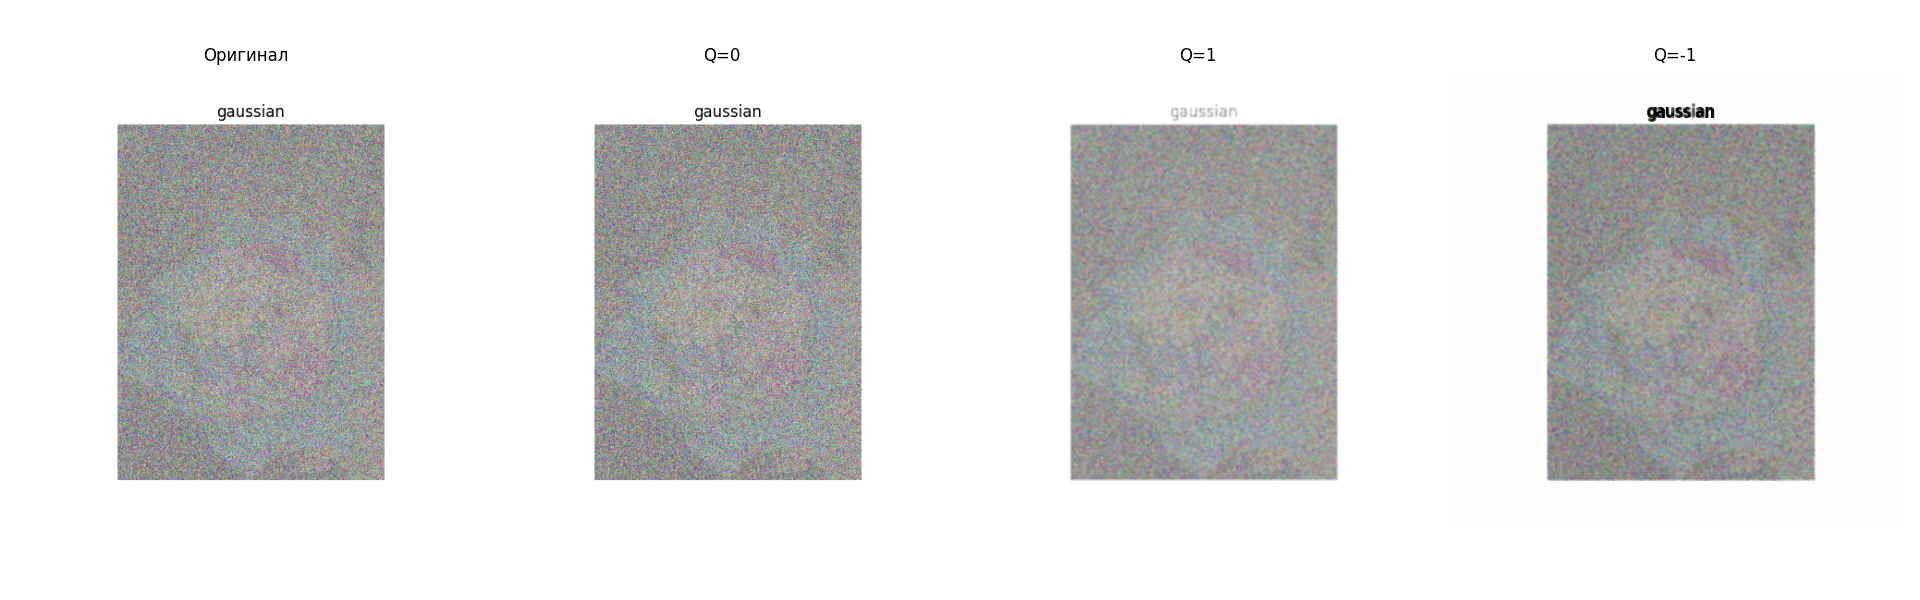
\includegraphics[width=1\linewidth]{../filtreted/kfGay.png}
	\end{figure}
	
	\item Шум квантования
	\begin{figure}[H]
		\centering
		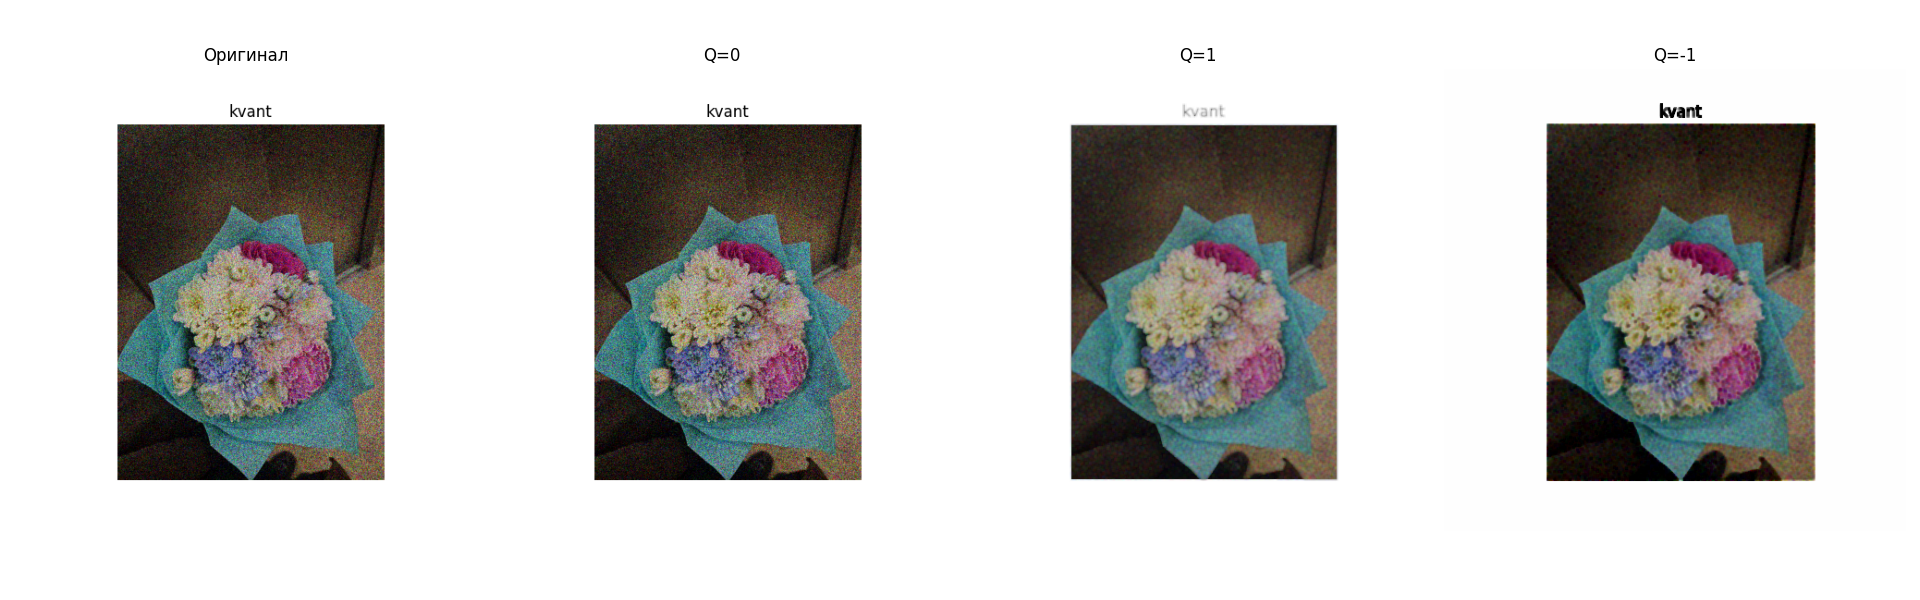
\includegraphics[width=1\linewidth]{../filtreted/kfKva.png}
	\end{figure}
\end{itemize}
	Фильтр эффективен против импульсного шума при правильном выборе Q, но усиливает гауссов и квантовый шумы.

\section{Task. Нелинейная фильтрация}

Мне нужно провести обработку искажённых изображений разными нелинейными фильтрами: 
медианным, взвешенным медианным, ранговым, винеровским и адаптивным медианным. 
Поэкспериментировать с размерами масок и параметрами фильтров.


\subsection{Медианная фильтрация}

Нелинейный метод обработки изображений, удаляющий импульсный шум ("соль-и-перец") с сохранением границ. Для каждого пикселя анализируется окрестность $k \times k$, значения сортируются, и центральному пикселю присваивается медиана:

\[ \text{median} = x_{\left\lceil \frac{k^2}{2} \right\rceil} \]

Реализация в OpenCV:
\begin{lstlisting}[language=python, caption={Медианная фильтрация}]
filtered = cv2.medianBlur(image, Q)
\end{lstlisting}
	
Применю фильтрацию к своим зашумленным изображениям. Возьму \( Q \in \{1, 3, 7\} \).

\begin{itemize}
	\item Импульсный шум
	\begin{figure}[H]
		\centering
		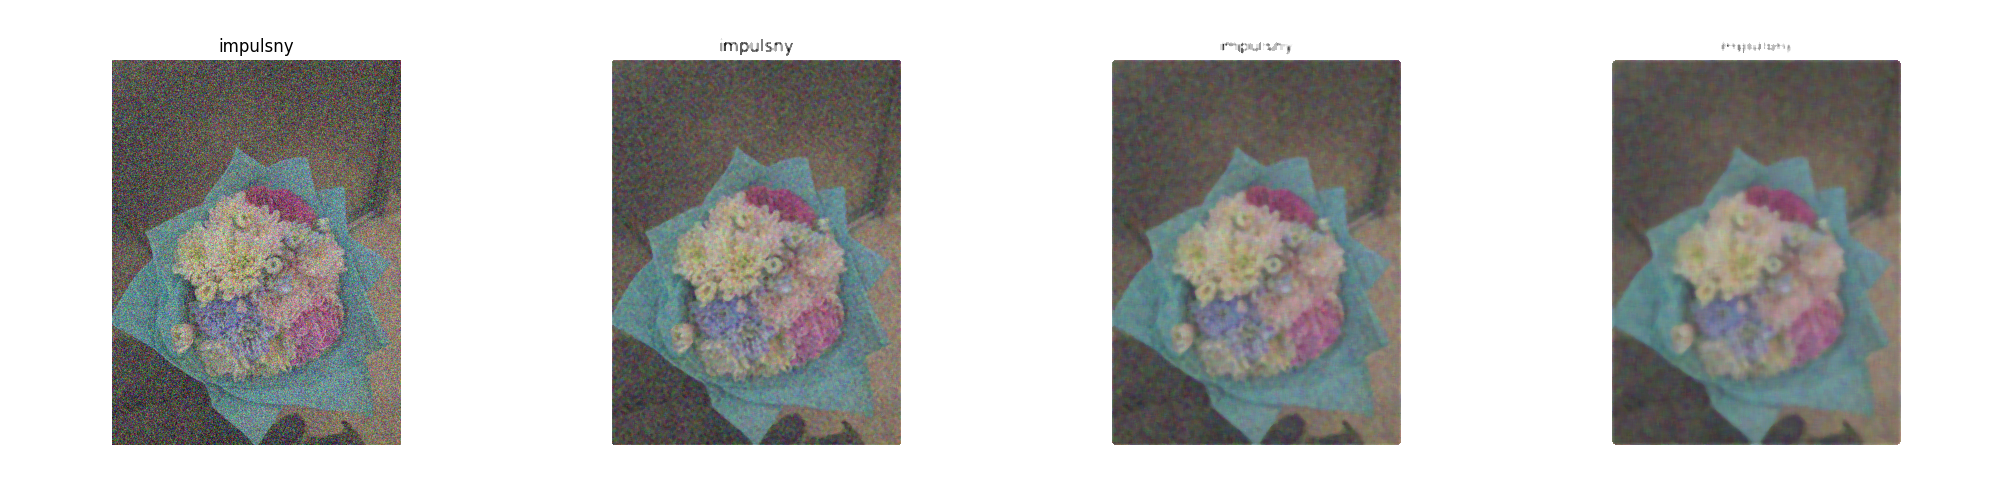
\includegraphics[width=1\linewidth]{../filtreted3/median/Fimpuls.png}
	\end{figure}
	
	\item Аддитивный шум
	\begin{figure}[H]
		\centering
		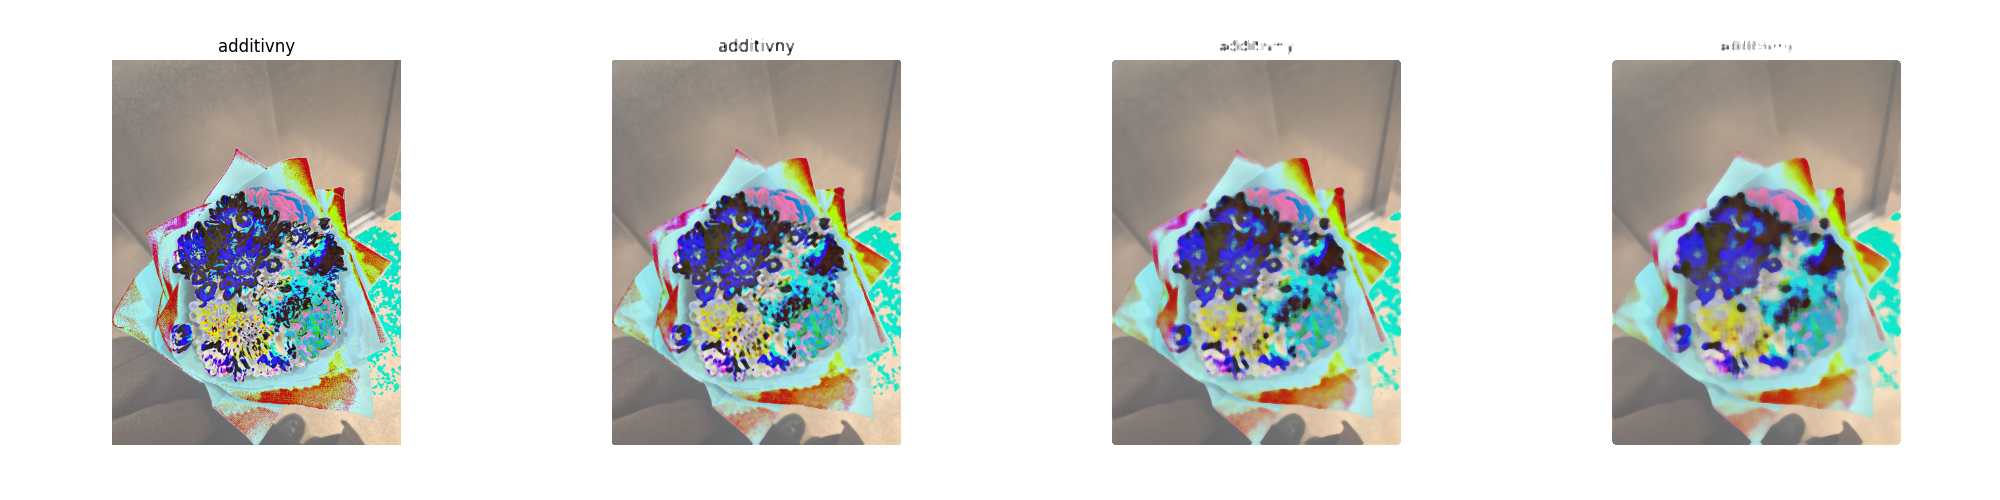
\includegraphics[width=1\linewidth]{../filtreted3/median/Fadditive.png}
	\end{figure}
	
	\item Мультипликативный шум
	\begin{figure}[H]
		\centering
		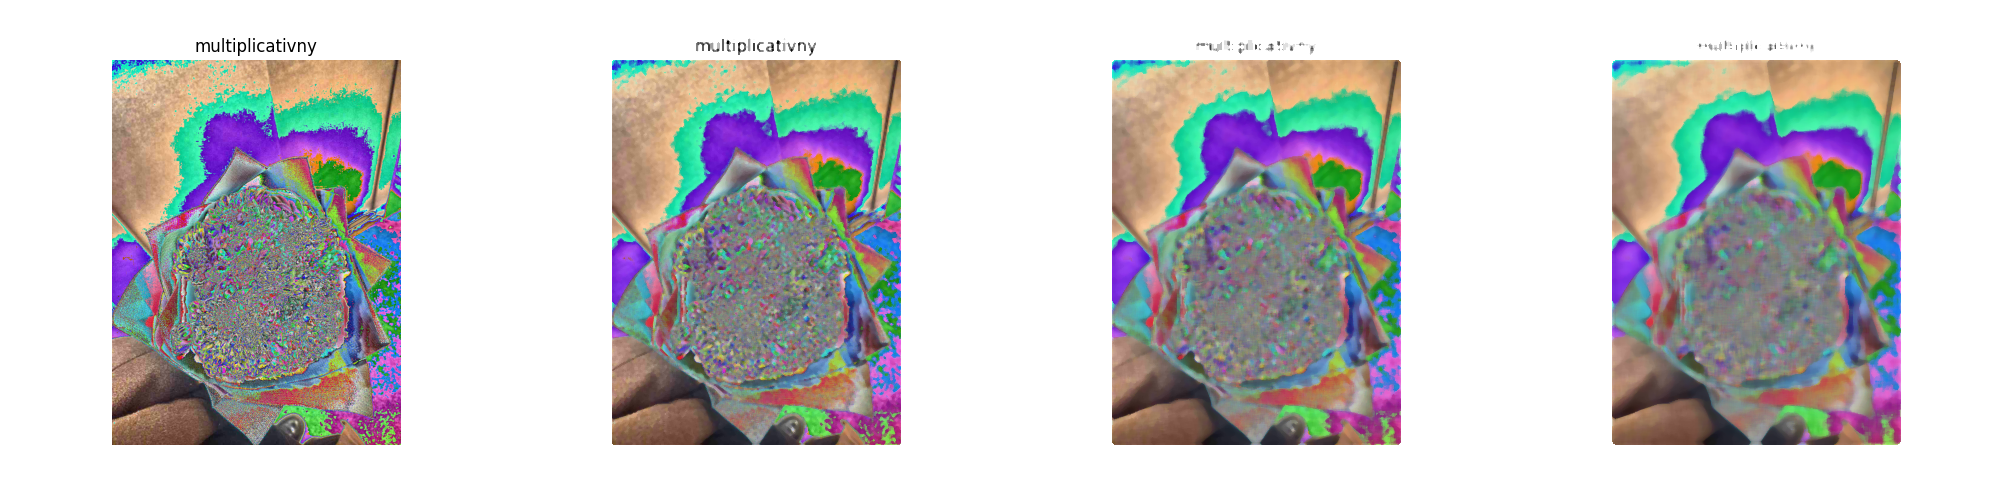
\includegraphics[width=1\linewidth]{../filtreted3/median/Fmultiplicativny.png}
	\end{figure}
	
	\item Шум гаусса
	\begin{figure}[H]
		\centering
		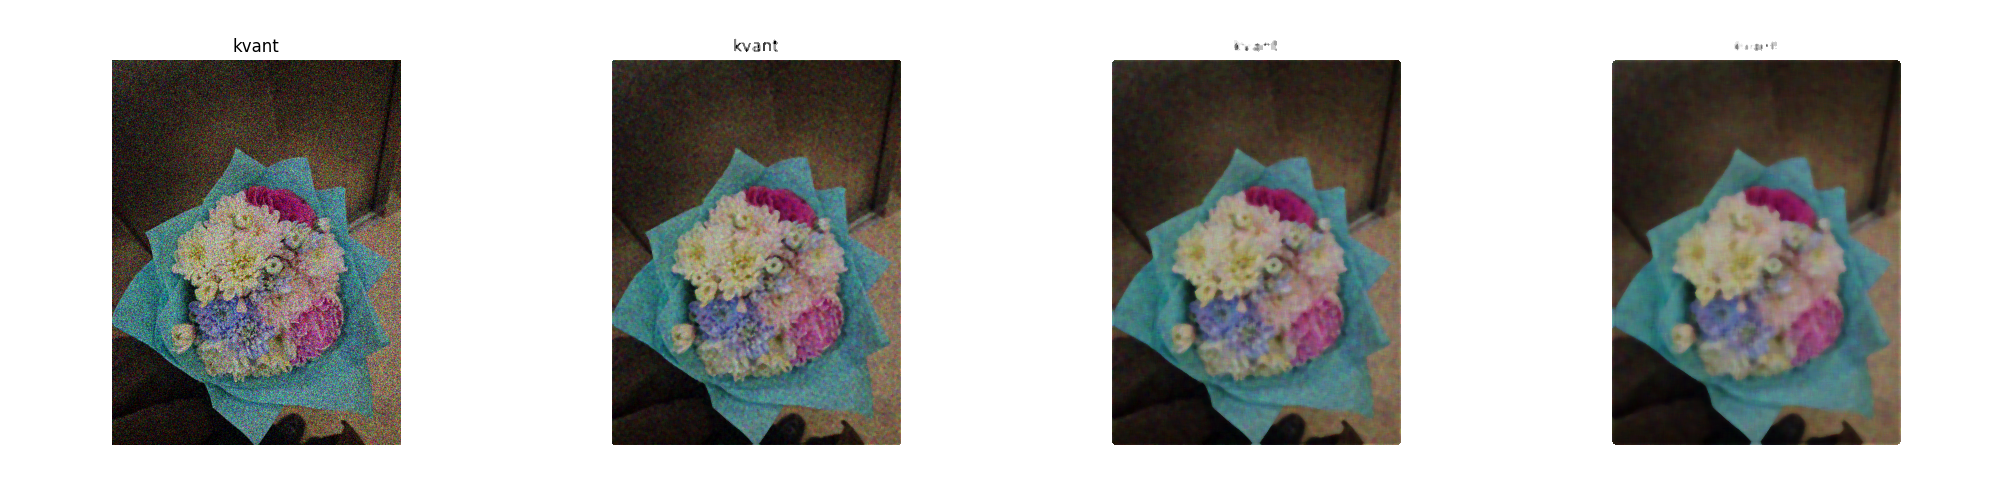
\includegraphics[width=1\linewidth]{../filtreted3/median/Fkvant.png}
	\end{figure}
	
	\item Шум квантования
	\begin{figure}[H]
		\centering
		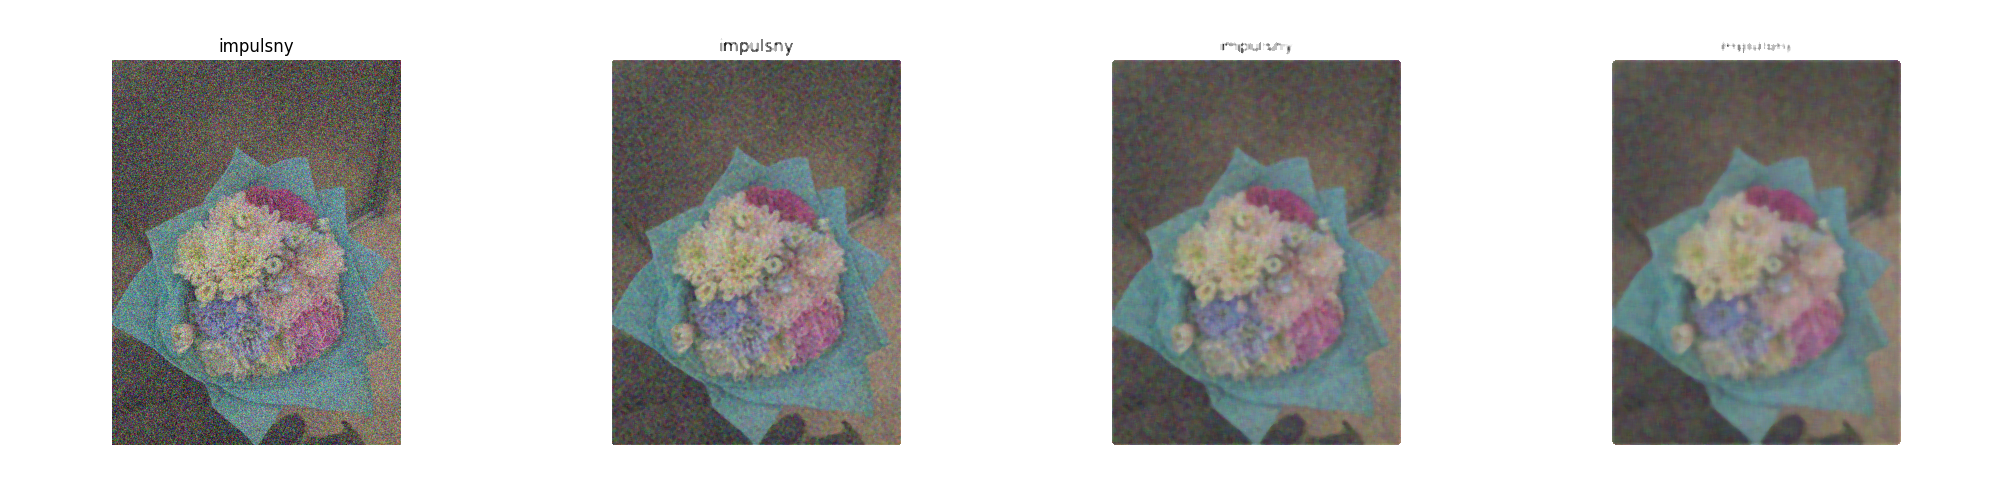
\includegraphics[width=1\linewidth]{../filtreted3/median/Fimpuls.png}
	\end{figure}
\end{itemize}	
	
	Медианный фильтр неплох для устранения импульсного шума, но неприменим для гауссова. 
	Оптимальное ядро~--- $3\times3$. Сохраняет границы, но размывает текстуры при увеличении ядра.
	
	
	\subsection{Взвешенная медианная фильтрация}
	
	
	Модификация медианного фильтра, где центральные пиксели окрестности имеют больший вес. Формула вычисления:
	
	\[
	I_{out}(x,y) = \mathrm{median}\{ \underbrace{I(x+i,y+j)}_{\text{повторяется } w_{ij} \text{ раз}} \}
	\]
	
Код:

\begin{lstlisting}[language=python, caption={Взвешенная медианная фильтрация}]
def weightedMedianFilter(inputImage, kernelSize=3, weightMatrix=None):
	if len(inputImage.shape) == 3:
		b, g, r = cv2.split(inputImage)
		bFiltered = weightedMedianFilter(b, kernelSize, weightMatrix)
		gFiltered = weightedMedianFilter(g, kernelSize, weightMatrix)
		rFiltered = weightedMedianFilter(r, kernelSize, weightMatrix)
		return cv2.merge([bFiltered, gFiltered, rFiltered])
	else:
		if weightMatrix is None:
			weightMatrix = np.ones((kernelSize, kernelSize), dtype=np.float32)
		
		pad = kernelSize // 2
		paddedImage = cv2.copyMakeBorder(inputImage, pad, pad, pad, pad, cv2.BORDER_REFLECT)
		outputImage = np.zeros_like(inputImage, dtype=np.uint8)
		
		for y in range(pad, paddedImage.shape[0] - pad):
			for x in range(pad, paddedImage.shape[1] - pad):
			neighborhood = paddedImage[y-pad:y+pad+1, x-pad:x+pad+1]
			weightedPixels = []
			for i in range(kernelSize):
				for j in range(kernelSize):
				weightedPixels.extend([neighborhood[i, j]] * int(weightMatrix[i, j]))
			outputImage[y-pad, x-pad] = np.median(weightedPixels)
		
		return outputImage
\end{lstlisting}
	
	
	Применю фильтрацию к своим зашумленным изображениям. Возьму \( Q \in \{1, 3, 9\} \).
	
	\begin{itemize}
		\item Импульсный шум
		\begin{figure}[H]
			\centering
			
\includegraphics[width=1\linewidth]{../filtreted3/weightedMedianFilter/Fimpuls.png}
		\end{figure}
		
		\item Аддитивный шум
		\begin{figure}[H]
			\centering
			
\includegraphics[width=1\linewidth]{../filtreted3/weightedMedianFilter/Fadditive.png}
		\end{figure}
		
		\item Мультипликативный шум
		\begin{figure}[H]
			\centering
			
\includegraphics[width=1\linewidth]{../filtreted3/weightedMedianFilter/Fmultiplicativny.png}
		\end{figure}
		
		\item Шум гаусса
		\begin{figure}[H]
			\centering
			
\includegraphics[width=1\linewidth]{../filtreted3/weightedMedianFilter/Fkvant.png}
		\end{figure}
		
		\item Шум квантования
		\begin{figure}[H]
			\centering
			
\includegraphics[width=1\linewidth]{../filtreted3/weightedMedianFilter/Fimpuls.png}
		\end{figure}
	\end{itemize}	
	
	
	Удалось избавится от импульсного, гауссовского и шума квантования, не без размытия при увеличении $Q$.
	
	
	\subsection{Ранговый фильтр}
	
	Ранговый фильтр~--- обобщение медианной фильтрации, где вместо медианы выбирается элемент с заданным порядковым номером $r$ в отсортированном векторе значений из окрестности:
	
	\[
	I_{out}(x,y) = \text{sort}(I_{window})[r]
	\]
	
	\begin{itemize}
		\item При $r = \lfloor N/2 \rfloor$ получаем классический медианный фильтр
		\item При $r=1$~--- фильтр минимума (эффективен против "перца")
		\item При $r=N$~--- фильтр максимума (эффективен против "соли")
	\end{itemize}
	
	Реализация:
\begin{lstlisting}[language=python, caption={Ранговая фильтрация}]
def rankFilter(inputImage, kernelSize=(3, 3), rank=4):
	if inputImage.dtype == np.uint8:
		inputImage = inputImage.astype(np.float32) / 255
	
	rows, cols = inputImage.shape[0], inputImage.shape[1]
	padY = (kernelSize[0] - 1) // 2
	padX = (kernelSize[1] - 1) // 2
	padded = cv2.copyMakeBorder(inputImage, padY, padY, padX, padX, cv2.BORDER_REPLICATE)
	
	if inputImage.ndim == 2:
		layers = np.zeros((rows, cols, kernelSize[0]*kernelSize[1]), dtype=np.float32)
		for i in range(kernelSize[0]):
			for j in range(kernelSize[1]):
				layers[:, :, i*kernelSize[1]+j] = padded[i:i+rows, j:j+cols]
	else:
		layers = np.zeros((rows, cols, inputImage.shape[2], kernelSize[0]*kernelSize[1]), dtype=np.float32)
		for i in range(kernelSize[0]):
			for j in range(kernelSize[1]):
				layers[:, :, :, i*kernelSize[1]+j] = padded[i:i+rows, j:j+cols, :]
	
	layers.sort()
	
	if inputImage.ndim == 2:
		return layers[:, :, rank]
	else:
		return layers[:, :, :, rank]
\end{lstlisting}
	
	
Применю фильтрацию к своим зашумленным изображениям. Возьму различные \texttt{kernelSize = (3 x 3), (5 x 5), (7 x 7), }
\begin{itemize}
	\item Импульсный шум
	\begin{figure}[H]
		\centering
		
\includegraphics[width=1\linewidth]{../filtreted3/rank/Fimpuls.png}
	\end{figure}
	
	\item Аддитивный шум
	\begin{figure}[H]
		\centering
		
\includegraphics[width=1\linewidth]{../filtreted3/rank/Fadditive.png}
	\end{figure}
	
	\item Мультипликативный шум
	\begin{figure}[H]
		\centering
		
\includegraphics[width=1\linewidth]{../filtreted3/rank/Fmultiplicativny.png}
	\end{figure}
	
	\item Шум гаусса
	\begin{figure}[H]
		\centering
		
\includegraphics[width=1\linewidth]{../filtreted3/rank/Fgaussian.png}
	\end{figure}
		
	\item Шум квантования
	\begin{figure}[H]
		\centering
		
\includegraphics[width=1\linewidth]{../filtreted3/rank/Fkvant.png}
	\end{figure}	
\end{itemize}
	
	Ранговый фильтр наиболее эффективен для борьбы с импульсным шумом, демонстрируя хорошие результаты при размере ядра 5×5. С увеличением размера ядра до 7×7 качество фильтрации улучшается, но появляется заметное размытие деталей. Для гауссова шума и шума квантования метод показывает ограниченную эффективность.
	
	
	\subsection{Винеровская фильтрация}
	
	
	Фильтр основан на минимизации среднеквадратической ошибки между исходным и восстановленным изображением.
	
	Реализация:
\begin{lstlisting}[language=python, caption={Винеровская фильтрация}]
def wienerFilter(inputImg, kernelSize=(7,7)):
	if inputImg.dtype == np.uint8:
		imgCopy = inputImg.astype(np.float32)/255
	else:
		imgCopy = inputImg.copy()
	
	rows, cols = inputImg.shape[:2]
	kernel = np.ones(kernelSize, np.float32)
	kPower = np.power(kernel, 2)
	padded = cv2.copyMakeBorder(imgCopy, 
								(kernelSize[0]-1)//2, kernelSize[0]//2,
								(kernelSize[1]-1)//2, kernelSize[1]//2,
								cv2.BORDER_REPLICATE)
	
	if len(inputImg.shape) == 3:
		bgrPlanes = cv2.split(padded)
		filteredPlanes = []
			for plane in bgrPlanes:
			planePower = np.power(plane, 2)
			m = np.zeros((rows, cols), np.float32)
			q = np.zeros((rows, cols), np.float32)
			
			for i in range(kernelSize[0]):
				for j in range(kernelSize[1]):
					m += kernel[i,j] * plane[i:i+rows, j:j+cols]
					q += kPower[i,j] * planePower[i:i+rows, j:j+cols]
				
			m /= np.sum(kernel)
			q /= np.sum(kernel)
			q -= m*m
			v = np.sum(q)/q.size
			
			planeFiltered = plane[(kernelSize[0]-1)//2:(kernelSize[0]-1)//2+rows,
			(kernelSize[1]-1)//2:(kernelSize[1]-1)//2+cols]
			planeFiltered = np.where(q < v, m, (planeFiltered-m)*(1-v/q) + m)
			filteredPlanes.append(planeFiltered)
		
		outputImg = cv2.merge(filteredPlanes)
	else:
		planePower = np.power(padded, 2)
		m = np.zeros((rows, cols), np.float32)
		q = np.zeros((rows, cols), np.float32)
		
		for i in range(kernelSize[0]):
			for j in range(kernelSize[1]):
				m += kernel[i,j] * padded[i:i+rows, j:j+cols]
				q += kPower[i,j] * planePower[i:i+rows, j:j+cols]
		
		m /= np.sum(kernel)
		q /= np.sum(kernel)
		q -= m*m
		v = np.sum(q)/q.size
		
		outputImg = padded[(kernelSize[0]-1)//2:(kernelSize[0]-1)//2+rows,
		(kernelSize[1]-1)//2:(kernelSize[1]-1)//2+cols]
		outputImg = np.where(q < v, m, (outputImg-m)*(1-v/q) + m)
	
	if inputImg.dtype == np.uint8:
		outputImg = np.clip(outputImg*255, 0, 255).astype(np.uint8)
	
	return outputImg
\end{lstlisting}
	
	Применю фильтрацию к своим зашумленным изображениям. Возьму различные \texttt{kernelSize = (3 x 3), (5 x 5), (7 x 7), }
	\begin{itemize}
		\item Импульсный шум
		\begin{figure}[H]
			\centering
			
\includegraphics[width=1\linewidth]{../filtreted3/wiener/Fimpuls.png}
		\end{figure}
		
		\item Аддитивный шум
		\begin{figure}[H]
			\centering
			
\includegraphics[width=1\linewidth]{../filtreted3/wiener/Fadditive.png}
		\end{figure}
		
		\item Мультипликативный шум
		\begin{figure}[H]
			\centering
			
\includegraphics[width=1\linewidth]{../filtreted3/wiener/Fmultiplicativny.png}
		\end{figure}
		
		\item Шум гаусса
		\begin{figure}[H]
			\centering
			
\includegraphics[width=1\linewidth]{../filtreted3/wiener/Fgaussian.png}
		\end{figure}
		
		
		\item Шум квантования
		\begin{figure}[H]
			\centering
			
\includegraphics[width=1\linewidth]{../filtreted3/wiener/Fkvant.png}
		\end{figure}
		
		Удалось улучшить изображения с испульсным шумом и шумом квантования.
			
	\end{itemize}
	
	\subsection{Адаптивная медианная фильтрация}
	
	Автоматически подбирает размер окна для каждого пикселя:
	\begin{itemize}
		\item Начинает с малого окна (3×3)
		\item Если медиана не подходит - увеличивает окно
		\item Максимальный размер задаётся параметром (7×7, 11×11 и т.д.)
	\end{itemize}

	
	
	Реализация:
	
\begin{lstlisting}[language=python, caption={Адаптивная медианная фильтрация}]
def adaptiveMedianFilter(inputImage, initialSize=3, maxSize=7):
	if len(inputImage.shape) == 3:
		inputImage = cv2.cvtColor(inputImage, cv2.COLOR_BGR2GRAY)
		
		pad = maxSize // 2
		paddedImage = cv2.copyMakeBorder(inputImage, pad, pad, pad, pad, cv2.BORDER_REFLECT)
		
		outputImage = np.zeros_like(inputImage)
		rows, cols = inputImage.shape
		
			for i in range(rows):
				for j in range(cols):
					x, y = i + pad, j + pad
					currentSize = initialSize
					
					while currentSize <= maxSize:
						half = currentSize // 2
						window = paddedImage[x-half:x+half+1, y-half:y+half+1]
						zMin = np.min(window)
						zMax = np.max(window)
						zMed = np.median(window)
						zXY = paddedImage[x, y]
						
						a1 = zMed - zMin
						a2 = zMed - zMax
						
						if a1 > 0 and a2 < 0:
							b1 = zXY - zMin
							b2 = zXY - zMax
							
							if b1 > 0 and b2 < 0:
								outputImage[i, j] = zXY
							else:
								outputImage[i, j] = zMed
								break
						else:
							currentSize += 2
					else:
						outputImage[i, j] = zXY
	
	return outputImage
\end{lstlisting}

	
	
\section{Task. Высокочастотная фильтрация}

В этом задании мне нужно обработать исходное изображение и выделить границы несколькими алгоритмами.

\begin{figure}[H]
	\centering
	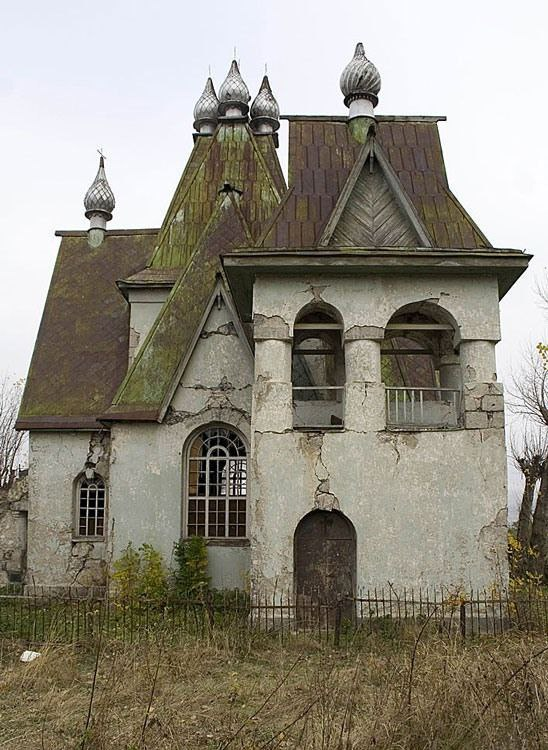
\includegraphics[width=0.5\linewidth]{../images/house.jpg}
	\caption{Исходное изображение}
\end{figure}

\subsection{Фильтр Робертса}
	
Фильтр Робертса:

\begin{equation*}
	G_x = \begin{bmatrix}1 & 0\\0 & -1\end{bmatrix},\ 
	G_y = \begin{bmatrix}0 & 1\\-1 & 0\end{bmatrix}
\end{equation*}

Градиент:
\begin{equation*}
	G = \sqrt{(I \ast G_x)^2 + (I \ast G_y)^2}
\end{equation*}

	
\begin{lstlisting}[language=python, caption={Фильтр Робертса}]
def robertsFilter(inputImage, threshold=None):
	if len(inputImage.shape) == 3:
		inputImage = cv2.cvtColor(inputImage, cv2.COLOR_BGR2GRAY)
	
	kernelX = np.array([[1, 0], 
						[0, -1]], dtype=np.float32)
	
	kernelY = np.array([[0, 1], 
						[-1, 0]], dtype=np.float32)
	
	gradX = cv2.filter2D(inputImage, -1, kernelX)
	gradY = cv2.filter2D(inputImage, -1, kernelY)
	
	outputImage = cv2.magnitude(gradX, gradY)
	outputImage = cv2.normalize(outputImage, None, 0, 255, cv2.NORM_MINMAX, cv2.CV_8U)
	
	_, outputImage = cv2.threshold(outputImage, threshold, 255, cv2.THRESH_BINARY)
	
	return outputImage
\end{lstlisting}	
		
	
\begin{figure}[H]
	\centering
	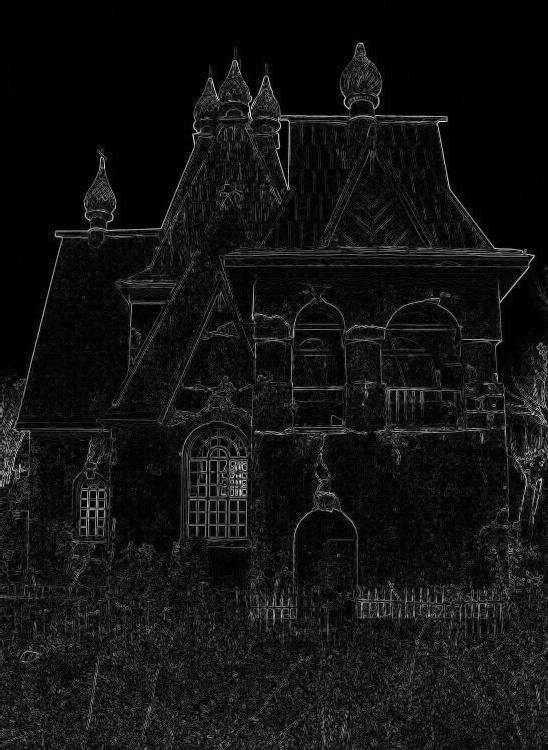
\includegraphics[width=0.5\linewidth]{../filtreted4/roberts.jpg}
	\caption{Изображение, обработанное фильтром Робертса}
\end{figure}	
	
	
	

\subsection{Фильтр Превитта}


Ядра для вычисления градиентов:
\[
G_x = \begin{bmatrix}
	-1 & 0 & 1 \\
	-1 & 0 & 1 \\
	-1 & 0 & 1
\end{bmatrix},\quad
G_y = \begin{bmatrix}
	-1 & -1 & -1 \\
	0 & 0 & 0 \\
	1 & 1 & 1
\end{bmatrix}
\]

Модуль градиента:
\[
G = \sqrt{(I * G_x)^2 + (I * G_y)^2}
\]
	
\begin{lstlisting}[language=python, caption={Фильтр Превитта}]
def prewittFilter(inputImage, threshold=None):
	if len(inputImage.shape) == 3:
		inputImage = cv2.cvtColor(inputImage, cv2.COLOR_BGR2GRAY)
	
	kernelX = np.array([[-1, 0, 1],
						[-1, 0, 1],
						[-1, 0, 1]], dtype=np.float32)
	
	kernelY = np.array([[-1, -1, -1],
						[0, 0, 0],
						[1, 1, 1]], dtype=np.float32)
	
	gradX = cv2.filter2D(inputImage, -1, kernelX)
	gradY = cv2.filter2D(inputImage, -1, kernelY)
	
	outputImage = np.sqrt(gradX**2 + gradY**2)
	outputImage = cv2.normalize(outputImage, None, 0, 255, cv2.NORM_MINMAX, cv2.CV_8U)
	
	_, outputImage = cv2.threshold(outputImage, threshold, 255, cv2.THRESH_BINARY)
	
	return outputImage
\end{lstlisting}	

\begin{figure}[H]
	\centering
	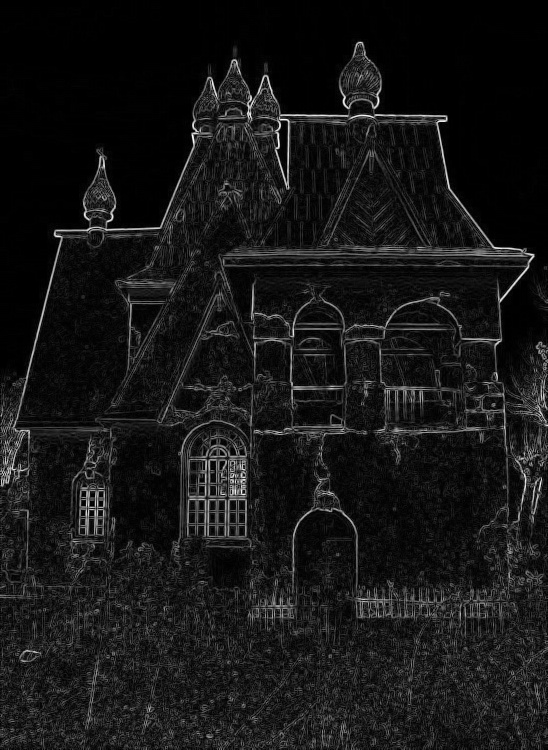
\includegraphics[width=0.5\linewidth]{../filtreted4/prewitt.jpg}
	\caption{Изображение, обработанное фильтром Превитта}
\end{figure}

\subsection{Фильтр Собела}


Ядра оператора:
\[
G_x = \begin{bmatrix} 
	-1 & 0 & 1 \\ 
	-2 & 0 & 2 \\ 
	-1 & 0 & 1 
\end{bmatrix},\quad
G_y = \begin{bmatrix} 
	1 & 2 & 1 \\ 
	0 & 0 & 0 \\ 
	-1 & -2 & -1 
\end{bmatrix}
\]

Модуль градиента:
\[
G = \sqrt{(I * G_x)^2 + (I * G_y)^2}
\]
\begin{lstlisting}[language=python, caption={Фильтр Собела}]
def sobelFilter(inputImage, threshold=None):
	if len(inputImage.shape) == 3:
		inputImage = cv2.cvtColor(inputImage, cv2.COLOR_BGR2GRAY)
	
	kernelX = np.array([[-1, 0, 1],
						[-2, 0, 2],
						[-1, 0, 1]], dtype=np.float32)
	
	kernelY = np.array([[1, 2, 1],
						[0, 0, 0],
						[-1, -2, -1]], dtype=np.float32)
	
	gradX = cv2.filter2D(inputImage, -1, kernelX)
	gradY = cv2.filter2D(inputImage, -1, kernelY)
	
	outputImage = np.sqrt(gradX**2 + gradY**2)
	outputImage = cv2.normalize(outputImage, None, 0, 255, cv2.NORM_MINMAX, cv2.CV_8U)
	
	if threshold is not None:
		_, outputImage = cv2.threshold(outputImage, threshold, 255, cv2.THRESH_BINARY)
	
	return outputImage
\end{lstlisting}	

\begin{figure}[H]
	\centering
	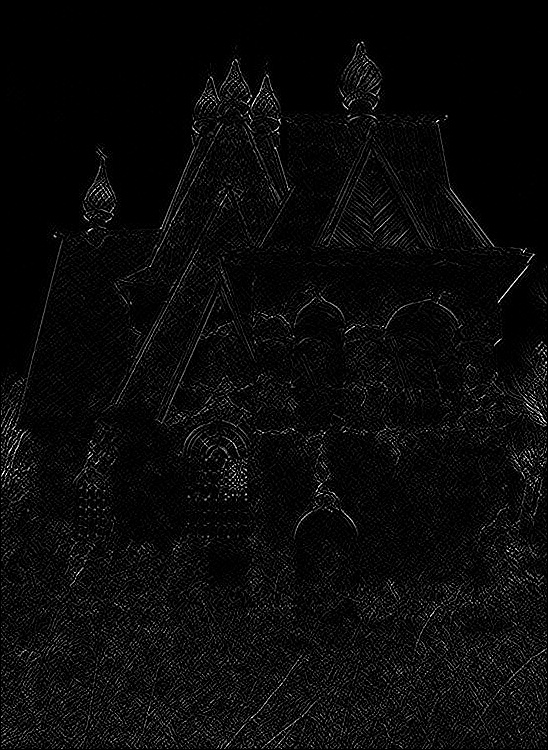
\includegraphics[width=0.5\linewidth]{../filtreted4/sobel.jpg}
	\caption{Изображение, обработанное фильтром Собела}
\end{figure}


\subsection{Фильтр Лапласса}
Оператор Лапласа:
\[
L(I(x,y)) = \frac{\partial^2 I}{\partial x^2} + \frac{\partial^2 I}{\partial y^2}
\]

Аппроксимация ядром:
\[
w_4 = \begin{bmatrix}
	0 & -1 & 0 \\
	-1 & 4 & -1 \\
	0 & -1 & 0
\end{bmatrix}
\]

\begin{lstlisting}[language=python, caption={Фильтр Лапласса}]
def laplacianFilter(img):
	kernel = np.array([[0, -1, 0],
	                   [-1, 4, -1],
	                   [0, -1, 0]])
	return cv2.filter2D(img, -1, kernel)
\end{lstlisting}	
	
\begin{figure}[H]
	\centering
	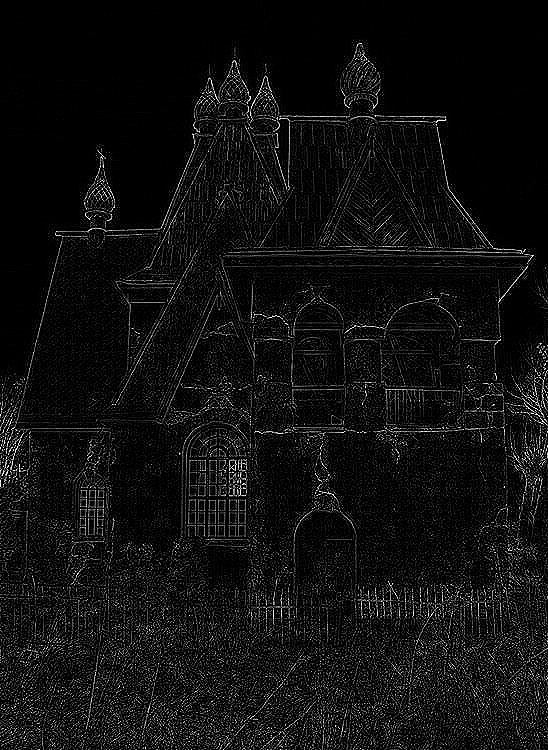
\includegraphics[width=0.5\linewidth]{../filtreted4/laplacian.jpg}
	\caption{Изображение, обработанное фильтром Лапласса}
\end{figure}

	
\subsection{Алгоритм Кенни}

Основные этапы:
\begin{enumerate}
	\item Гауссово размытие: $G_{\sigma} * I$
	\item Градиент: $\sqrt{G_x^2 + G_y^2}$ и $\theta = \arctan(G_y/G_x)$
	\item Подавление немаксимумов
	\item Гистерезис: $T_{low} = 50$, $T_{high} = 150$
\end{enumerate}
	
	
\begin{lstlisting}[language=python, caption={Алгоритм Кенни}]
def cannyEdge(img, low=50, high=150):
	if len(img.shape) == 3:
		img = cv2.cvtColor(img, cv2.COLOR_BGR2GRAY)
		
	edges = cv2.Canny(img, low, high)
	return edges.astype(np.uint8)
\end{lstlisting}
	

\begin{figure}[H]
	\centering
	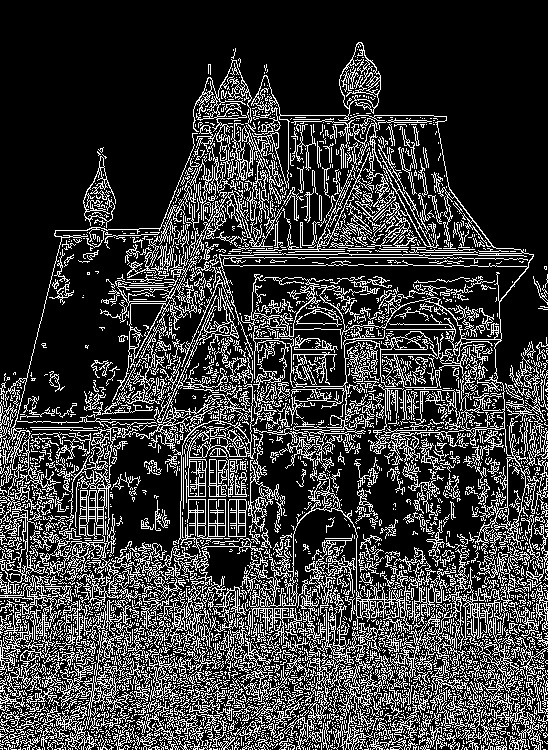
\includegraphics[width=0.5\linewidth]{../filtreted4/canny.jpg}
	\caption{Изображение, обработанное алгоритмом Кенни}
\end{figure}

	
	\section{Вопросы}
	
	
	\begin{enumerate}
		\item  В чем заключаются основные недостатки адаптивных методов фильтрации изображений?
		
		--- Адаптивные методы требуют больше вычислений, чувствительны к настройкам и могут создавать артефакты.
		
		\item При каких значениях параметра $Q$ контргармонический фильтр будет работать как арифметический, а при каких — как гармонический?
		
		--- При $Q = 0$ и $Q = -1$ соответственно.
		
		\item Какими операторами можно выделить границы на изображении?
		
		--- Операторами, рассмотренными в задании 4.
		
		\item Для чего на первом шаге выделения контуров, как правило, выполняется низкочастотная фильтрация?
		
		--- Низкочастотная фильтрация выполняется для подавления шумов и мелких деталей, чтобы улучшить качество последующего выделения контуров.
		
	\end{enumerate}
	
	\section{Вывод}
	
	Фильтр Гаусса эффективно устраняет высокочастотные шумы, однако приводит к заметному снижению резкости изображения. Медианная фильтрация демонстрирует высокую эффективность против импульсных шумов при сохранении чётких границ объектов. Адаптивные алгоритмы показывают наилучшие результаты обработки, но требуют больше вычислительных ресурсов. Для задач выделения границ оптимальным выбором является алгоритм Кэнни, обеспечивающий точность при правильной настройке параметров.
	
	Таким образом, выбор метода фильтрации должен основываться на анализе типа шума и требований к качеству обработки изображения.
	
	\href{https://github.com/decadeos/ITMO/tree/master/2_course/texViz/lab3}{GitHub}.
\end{document}